\documentclass[x11names, crop, tikz]{standalone}
\usetikzlibrary{shapes,arrows,chains, positioning}
\begin{document}
	% -------------------------------------------------
	% Set up a new layer for the debugging marks, and make sure it is on
	% top
	\pgfdeclarelayer{marx}
	\pgfsetlayers{main,marx}
	% A macro for marking coordinates (specific to the coordinate naming
	% scheme used here). Swap the following 2 definitions to deactivate
	% marks.
	\providecommand{\cmark}[2][]{%
		\begin{pgfonlayer}{marx}
			\node [nmark] at (c#2#1) {#2};
		\end{pgfonlayer}{marx}
	} 
	\providecommand{\cmark}[2][]{\relax} 
	% -------------------------------------------------
	% Start the picture
	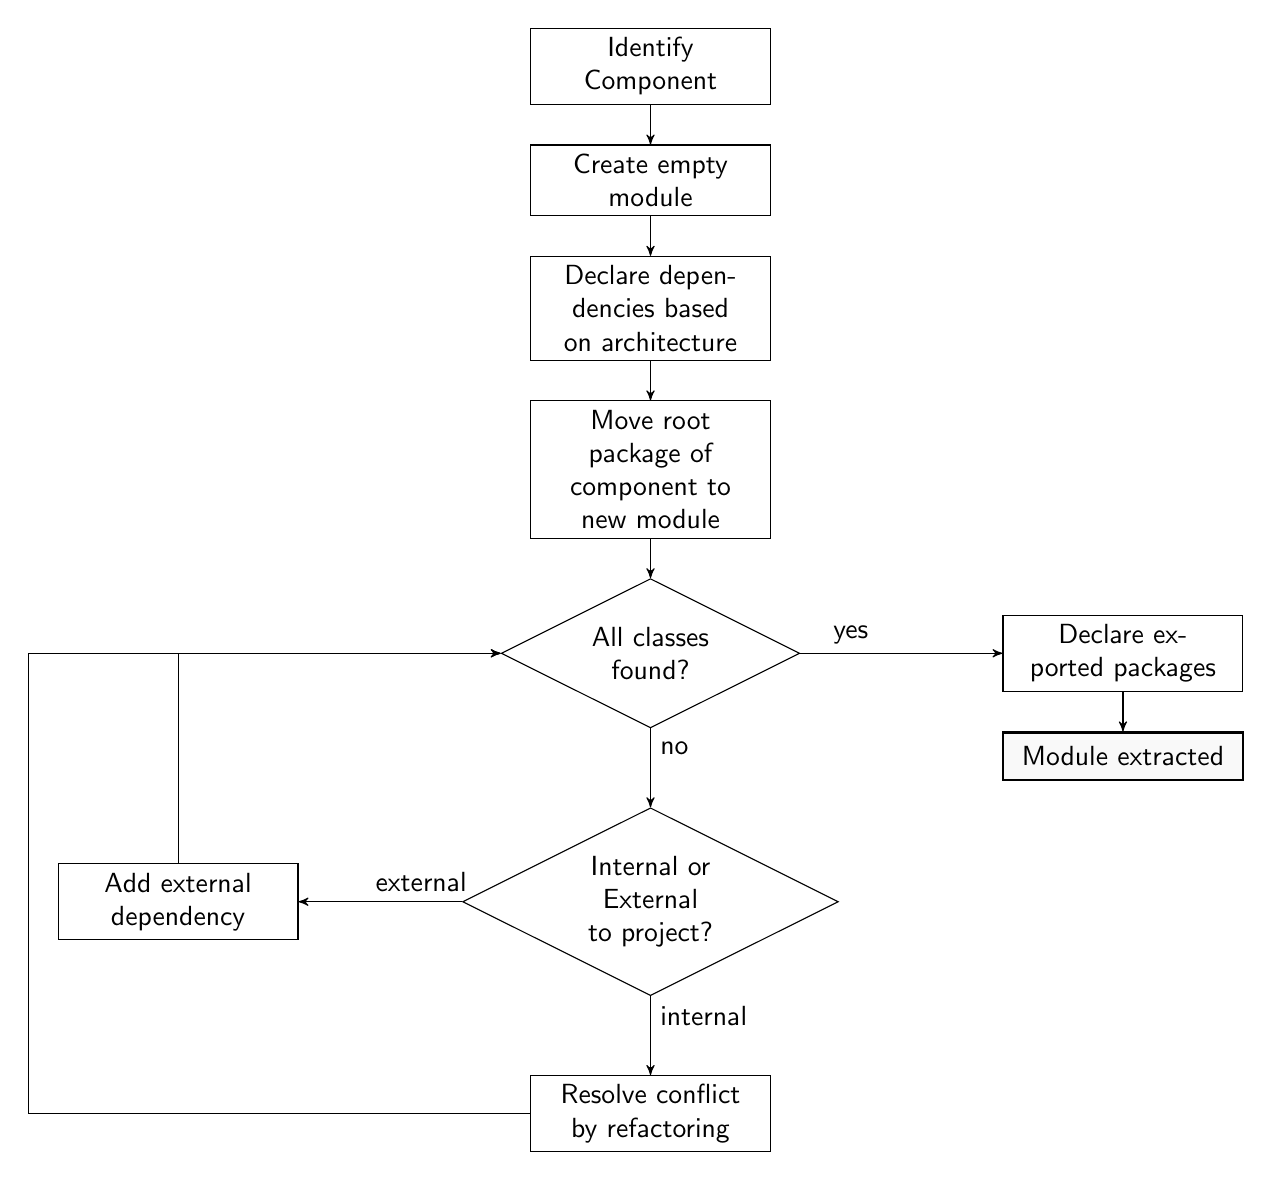
\begin{tikzpicture}[%
	every node/.style={font = \sffamily},
	>=stealth',              % Nice arrows; your taste may be different
	start chain=going below,    % General flow is top-to-bottom
	node distance=5mm and 60mm, % Global setup of box spacing
	every join/.style={norm},   % Default linetype for connecting boxes
	]
	% ------------------------------------------------- 
	% A few box styles 
	% <on chain> *and* <on grid> reduce the need for manual relative
	% positioning of nodes
	\tikzset{
		base/.style={draw, on chain, on grid, align=center, minimum height=4ex},
		proc/.style={base, rectangle, text width=8em},
		test/.style={base, diamond, aspect=2, text width=5em},
		term/.style={proc, rounded corners},
		% coord node style is used for placing corners of connecting lines
		coord/.style={coordinate, on chain, on grid, node distance=6mm and 25mm},
		% nmark node style is used for coordinate debugging marks
		nmark/.style={draw, cyan, circle, font={\sffamily\bfseries}},
		% -------------------------------------------------
		% Connector line styles for different parts of the diagram
		norm/.style={->, draw},
		free/.style={->, draw},
		cong/.style={->, draw},
		it/.style={font={\small\itshape}},
		final/.style={thick, fill=gray!5}
	}

	\node [proc]						(p1)	{Identify Component};
	\node [proc,join]							{Create empty module};
	\node [proc,join]							{Declare dependencies based on architecture};
	\node [proc,join]							{Move root package of component to new module};
	\node [test,join]					(t1)	{All classes found?};
	
	\node[proc, right=of t1]			(p2)	{Declare exported packages};
	\node[proc, join, final]					{Module extracted};
	
	\node[test, below=1cm of t1.south]	(t2)	{Internal or External to project?};
	
	\node[proc, left=of t2]				(p3)	{Add external dependency};
	
	\node[proc, below=1cm of t2.south]	(p4)	{Resolve conflict by refactoring};
	
	\draw[->] (t1) -- (p2) node[near start, above] {yes};
	\draw[->] (t1) -- (t2) node[near start, right] {no};
	
	\draw[->] (t2) -- (p3) node[near start, above] {external};
	\draw[->] (t2) -- (p4) node[near start, right] {internal};
	
	\draw[->] (p3) |- (t1);
	
	\coordinate[left=6cm of t1] (ctl);
	\draw[->] (p4) -| (ctl) -- (t1);

	\end{tikzpicture}
	% =================================================
\end{document}